\section{Experiments}
We apply the datasets from University of Virginia on both water and electricity disaggregation. 
There are totally six data sets. The statistic of these six data sets are listed in Table \ref{table_datasets}. 
Usually the interval of these datasets is 2 or 3 seconds. 
A sensor is instrumented on each device to record its operations. 
\begin{table}[!t]
\renewcommand{\arraystretch}{1.3}
\caption{Electricity Dataset}
\label{table_datasets}
\centering
\begin{tabular}{|c|c|c|c|}
\hline
Data sets & Start date & End date & Duration (day) \\
\hline
\hline
Study 10 & 02-10-2014 & 02-21-2014 & 12\\
\hline
Study 11 & 01-27-2014 & 02-07-2014 & 12\\
\hline
Study 12 & 01-09-2014 & 01-21-2014 & 12\\
\hline
Study 13 & 12-23-2013 & 01-03-2014 & 12\\
\hline
Study 14 & 12-09-2013 & 12-20-2013 & 12\\
\hline
Study 101 & 06-09-2014 & 06-28-2014 & 20\\
\hline
\end{tabular}
\end{table}

\subsection{Electricity Disaggregation}
For electricity data, we use aggregated data and the on/off events of the 
ground truth to extract the power levels of each device. 

In order to extract the power level of each device, 
we use a window size of $w=30s$ ahead and behind to match 
the aggregated data to the ground truth data.
%%Getting the time stamp from the ground truth of each device, 
%%then match the time of the aggregated data before $30s$ and after $30s$, 
If there is only one power change during these $1$ minute duration, 
this power level changes must come from this device. 
Usually, it takes around $2-5$ seconds for an electric device to reach
a steady power level  state. 
The on and off events reflect different duration of a device to 
turn to a steady state. 
Therefore, we measure the minimal duration of the on event and off event 
of each device. 

After we go over all the aggregated data and on/off events from the sensor data, 
we obtain the power levels of each device. 
By applying normal distribution to the positive figures and negative figures 
separately, we compute the mean value of the on/off event and
get the power levels of each electric device. 
The power levels and duration of each device are listed in Table \ref{table_study10results}.
\begin{table*}[!t]
\renewcommand{\arraystretch}{1.3}
\caption{Power Levels, Standard Deviation of Power Levels, On/off Duration, Connected Phases and Disaggregation Results of Electricity Devices from Study10.}
\label{table_study10results}
%\tbl{Power Levels, Standard Deviation of Power Levels, On/off Duration, Connected Phases and Disaggregation Results of Electricity Devices from Study10.\label{table_study10results}}{
\centering
%\small
\footnotesize
%\scriptsize
\setlength\tabcolsep{2pt}
\begin{tabular}{|c|c|c|c|c|c|c|c|c|c|c|}
\hline
\multirow{2}{*}{Device} & Power & Standard & On/off &  \multirow{2}{*}{Phase} & \multicolumn{3}{|c|}{Recursive Multivariate Motif Mining} & \multicolumn{3}{|c|}{AFAMAP}\\
\cline{6-11}
           &  Levels & Deviation & Duration &  &Precision&  Recall &  F-measure & Precision & Recall & F-measure\\ 
\hline
\hline
\multirow{2}{*}{HeatingIndoor+} & \multirow{2}{*}{10590W} & \multirow{2}{*}{1270W} & \multirow{2}{*}{60s} & \multirow{2}{*}{1+2} & \multirow{2}{*}{0.979} & \multirow{2}{*}{0.928} & \multirow{2}{*}{0.953} & \multirow{2}{*}{0.870}& \multirow{2}{*}{0.45} & \multirow{2}{*}{0.598}\\
HeatingOutdoor &  &  &  &  &  &  &  &  & & \\
\hline
Waterheater & 4450W & 350W &  2-5s & 1+2 & 0.999 & 0.997 &0.998 &0.627& 0.882 &0.733\\
\hline
Humidifier & 1470W & 90W & 10s & 1 & 0.997 & 0.992 &0.995 & 0.725 & 0.858 & 0.787\\
\hline
Microwave & 1850W & 200W & 10s & 2 & 0.95 &0.758 & 0.843 & 0.032 & 0.819 & 0.06\\
%\hline
%HeatingOutdoor & 4446W & 140 W & 2-18s & 1+2 &0.308 & 0.66& 0.42& & &\\
\hline
\multirow{2}{*}{Dryer} & 5200W &400W & 2-5s & 1+2 & \multirow{2}{*}{0.911}&\multirow{2}{*}{0.996}&\multirow{2}{*}{0.952}& \multirow{2}{*}{0.011}&\multirow{2}{*}{0.561} & \multirow{2}{*}{0.021}\\
\cline{2-3} \cline{4-5}
                       & 875W &225W  & 2-5s & 1 & & & & & &\\
%\hline
%L007 & 239W & 56W &  2-5s &2 & & & & & &\\
%\hline
%Fridge & 102W & 68W & 2-5s &1& - & - & - & & &\\
%\line
%L010 & 92W & 16W & 2-5s &2& & & & & &\\
%\cline
%L011 & 117W & 29W & 2-5s &1& & & & & &\\
%\hline
%L012 & 104W & 28W & 2-5s & 2& & & & & &\\
\hline
\end{tabular}
%}
\end{table*}

By analyzing each device, we notice that sometimes the power levels and 
on/off duration are insufficient to identify the electric devices. 
For instance, it takes $2-5$ seconds for the device heatingIndoor to reach a steady state after starting,
as shown in Figure \ref{fig_heatingDevices} (a).
But when the combined device of heatingIndoor and heatingOutdoor 
starts, the starting duration takes around $4-18$ seconds. 
As shown in Figure \ref{fig_patterns} (b), before reaching a relatively stable state. 
the power levels rapidly change 9 times within 15 seconds after this combined device starts
If we accumulate these power levels together, it's not a fix number. Therefore, for this kind of device, 
we can only compare the shape of the startup to decide the on events 
from the aggregated data. 
%\begin{figure*}[!t]
        \centering{
                \begin{tabular}{cccccc}
                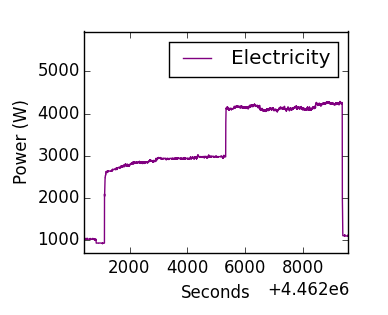
\includegraphics[width=2.1in]{multidisaggfig/heatingIndoorOutdoorPattern1_sum.png}&
                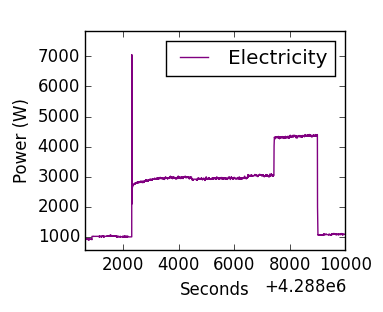
\includegraphics[width=2.1in]{multidisaggfig/heatingIndoorOutdoorPattern2_sum.png}&
                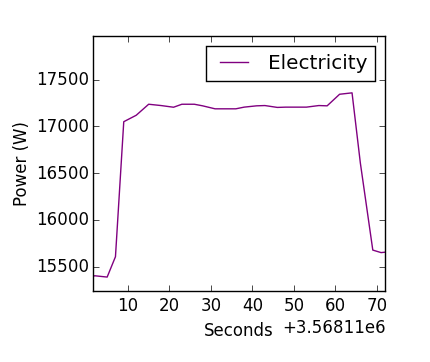
\includegraphics[width=2.1in]{multidisaggfig/microwave_sum.png}\tabularnewline
                (a) & (b)&(c)\tabularnewline
                 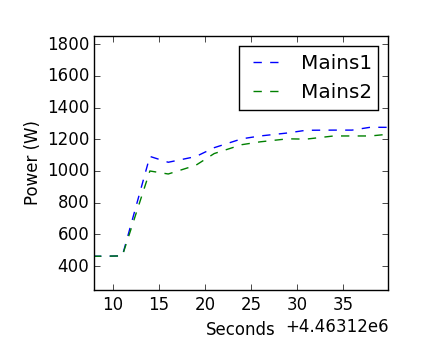
\includegraphics[width=2.1in]{multidisaggfig/heatingIndoorOutdoorPattern1.png}&
                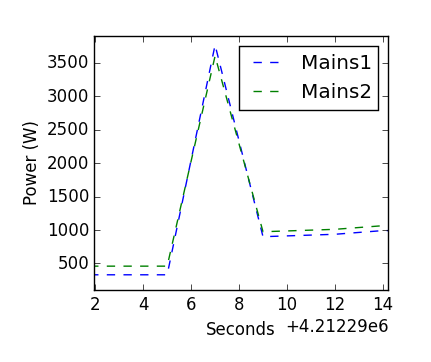
\includegraphics[width=2.1in]{multidisaggfig/heatingIndoorOutdoorPattern2.png}&
                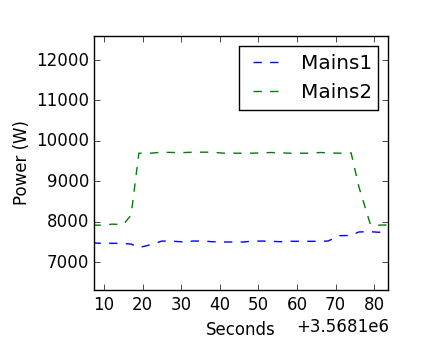
\includegraphics[width=2.1in]{multidisaggfig/microwave.png}\tabularnewline
                (d) & (e)&(f)\tabularnewline
                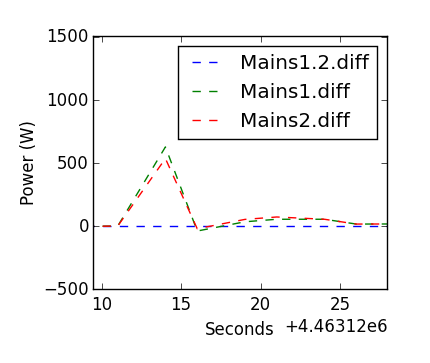
\includegraphics[width=2.1in]{multidisaggfig/heatingIndoorOutdoorPhase12On_1.png}&
                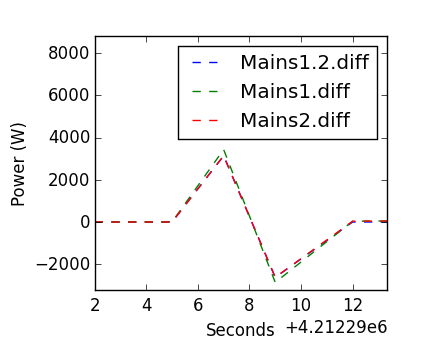
\includegraphics[width=2.1in]{multidisaggfig/heatingIndoorOutdoorPhase12On_2.png}&
                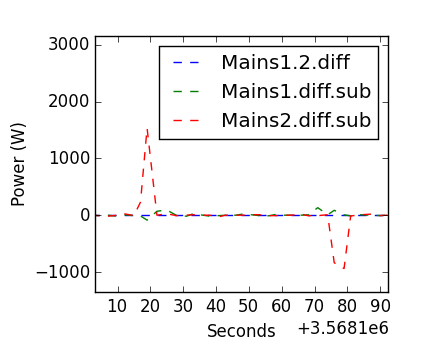
\includegraphics[width=2.1in]{multidisaggfig/microwavePhase2OnOff.png}\tabularnewline
               (g)&(h)&(i)\tabularnewline
                \end{tabular}
                }
        \caption{
       Devices (a) heatingIndoorOutdoor (b) heatingIndoorOutdoor (another pattern) (c) microwave in the aggregated power of sum of mains1 and main2. 
       Devices (d) heatingIndoorOutdoor (e) heatingIndoorOutdoor (another pattern) (f) microwave in the aggregated power of mains1 and main2. 
       Devices (g) heatingIndoorOutdoor (h) heatingIndoorOutdoor (another pattern) (i) microwave in the diffs data of aggregated power of mains1 and main2. 
       Since all of them starts synchronously in two mains, they are disaggregated by multivariate piecewise motif mining.  
}
        \label{fig_patterns}
\end{figure*}

We apply both episode mining and dynamic time warping approach on these six datasets. 
At first, we find those devices which can be found by episode mining. 
Then we use dynamic time warping to disaggregate the device indoorOutdoor unit. 
The precision and recall results on the data set study 10 are listed in Table \ref{table_study10results}.

The experiments results on the heatingIndoor are shown in Figure \ref{fig_heatingIndoorResults}.
The on event of heatingIndoor lasts for around 10 seconds and the off event 50 seconds. 
the power changes twice consecutively.  
For both on/off events, 
since each time the power changes more than $80W$, which is defined by us, 
these two power changes are merged as one device. 
Figure \ref{fig_heatingIndoorResults} (c) illustrates the disaggregated heatingIndoor device 
over a period of time. 
\begin{figure*}[!t]
        \centering{
                \begin{tabular}{cc}
                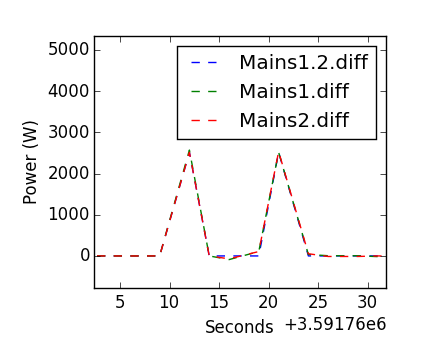
\includegraphics[width=0.5\textwidth]{multidisaggfig/heatingIndoorPhase12On.png} &
                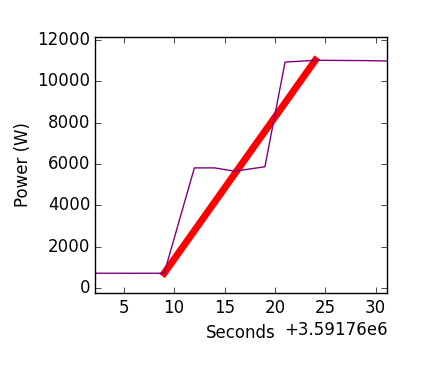
\includegraphics[width=0.5\textwidth]{multidisaggfig/heatingIndoorUp.png}\tabularnewline
                (a) & (b) \tabularnewline
                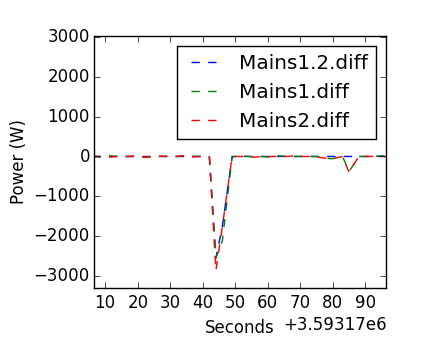
\includegraphics[width=0.5\textwidth]{multidisaggfig/heatingIndoorPhase12Off.png} &
                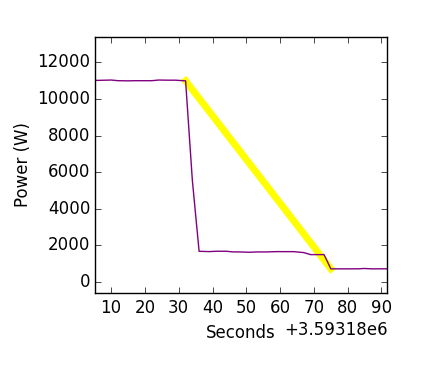
\includegraphics[width=0.5\textwidth]{multidisaggfig/heatingIndoorDown.png}\tabularnewline
                (c) & (d) \tabularnewline
                \end{tabular}
                }
        \caption{
        (a) On piecewise event and (c) Off piecewise event of heatingIndoor. heatingIndoor is disaggregated by motif mining the on event (b) and off event (d).}
        \label{fig_heatingIndoorResults}
\end{figure*}

\begin{figure*}[!t]
        \centering{
                \begin{tabular}{cccc}
                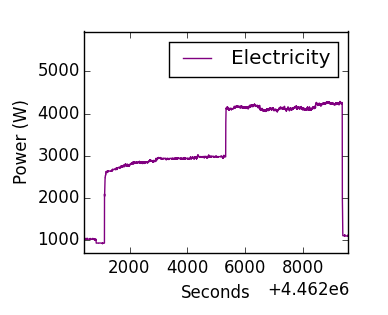
\includegraphics[width=3.2in]{multidisaggfig/heatingIndoorOutdoorPattern1_sum.png} &
                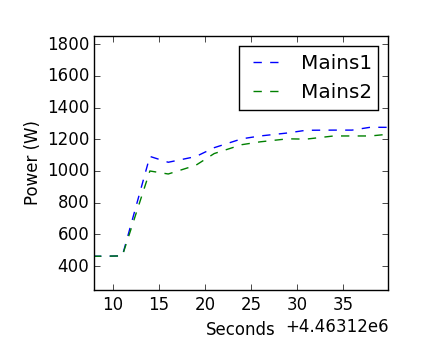
\includegraphics[width=3.2in]{multidisaggfig/heatingIndoorOutdoorPattern1.png} \tabularnewline
                 (a) & (b)\tabularnewline
                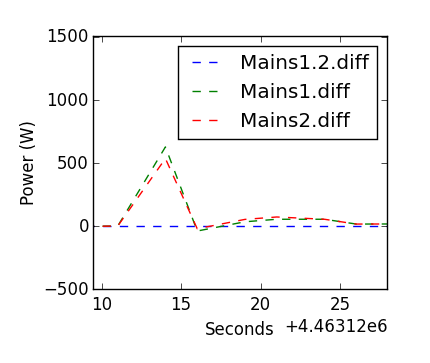
\includegraphics[width=3.2in]{multidisaggfig/heatingIndoorOutdoorPhase12On_1.png} &
                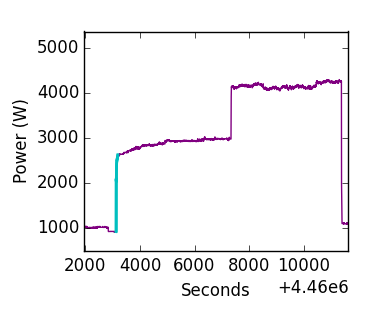
\includegraphics[width=3.2in]{multidisaggfig/heatingIndoorOutdoorFittedPattern1.png}\tabularnewline
                (c) &(d) \tabularnewline
                \end{tabular}
                }
        \caption{
        Disaggregating continuous variable load heating outdoor. 
        (a) the startup in the sum of aggregated power (b) the startup in two phases (c) the diffs in two phases (d) the disaggregated on event of heating outdoor.}
        \label{fig_heatingOutdoorResults}
\end{figure*}

%\input{fig/humidifierResults}
 
%The on event of heating indoor and outdoor is hard to be found by searching the power levels and duration because it is a continuous variable load. 
%We extract the vector event of on event of this device and compute its differential time series over around 50 seconds. 
%There are two patterns as shown in Figure \ref{fig_patterns} (e) and (f).
%Then we do dynamic time warping subsequence search to figure out the on events. 
%The Figure \ref{fig_dtwHeatingIndoorOutdoor} (a), (b) and (c) displays two matched patterns. 
%and the matched patterns for some time. 
%Note that the off event of heating indoor and outdoor lasts for several seconds with power levels ranging from 1700W to 2100W. 
%We still use motif mining approach to disaggregate this device. 
%\begin{figure*}[!t]
        \centering{
                \begin{tabular}{ccc}
                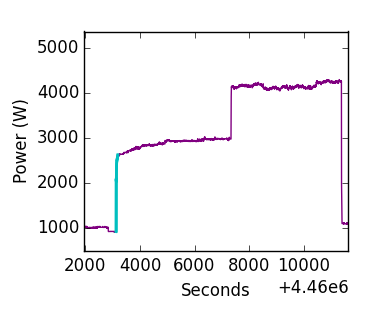
\includegraphics[width=2.1in]{multidisaggfig/heatingIndoorOutdoorFittedPattern1.png}&
                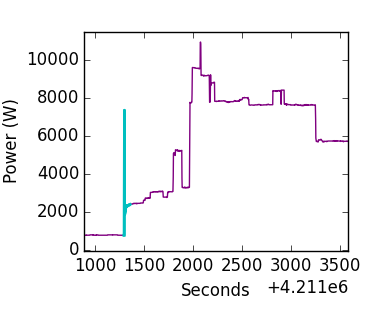
\includegraphics[width=2.1in]{multidisaggfig/heatingIndoorOutdoorFittedPattern2.png}&
                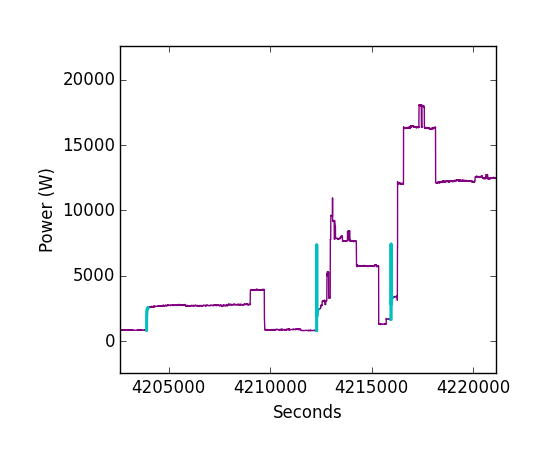
\includegraphics[width=2.1in]{multidisaggfig/heatingIndoorOutdoorFittedSnippet.png}
                \tabularnewline
                (a) & (b) & (c) \tabularnewline
                \end{tabular}
                }
        \caption{
        (a) \& (b): two different patterns fitted of heating indoor and outdoor. (c) snippet of on event of heating indoor and outdoor over a period of time}
        \label{fig_dtwHeatingIndoorOutdoor}
\end{figure*}

%We apply the same approach to other data sets. 
%.......

